\documentclass[12pt,titlepage]{article}

% \usepackages21{fancyhdr}

\usepackage[printwatermark]{xwatermark}

\usepackage{grffile}
\usepackage{xcolor}
\usepackage{lipsum}
\usepackage{times}
\usepackage{soul}
\usepackage{epsfig}
\usepackage{rotating}
\usepackage{url}
\usepackage{latexsym}
\usepackage{graphicx}
\usepackage{amsfonts}
\usepackage{amsmath, amsthm, amssymb}
\usepackage{fullpage}
\usepackage{setspace}
\usepackage{natbib}
\usepackage{longtable}
\usepackage{keyval}
\usepackage{caption,subcaption}
\usepackage{arydshln}
%%\usepackage[hyphenbreaks]{breakurl}

%% allow urls to get broken on hyphens
\usepackage{hyperref}
\def\UrlBreaks{\do\/\do-}


%% APSR submission: no commas in citations between name and year
%% See http://merkel.zoneo.net/Latex/natbib.php
\bibpunct{(}{)}{;}{author-year}{}{;}

% the opening bracket symbol, default = (
% the closing bracket symbol, default = )
% the punctuation between multiple citations, default = ;
% the letter `n' for numerical style, or `s' for numerical superscript style, any other letter for author-year, default = author-year;
% the punctuation that comes between the author names and the year
% the punctuation that comes between years or numbers when common author lists are suppressed (default = ,);

\usepackage{footmisc}
\renewcommand{\footnotelayout}{\doublespacing} % set spacing in footnotes
\newlength{\myfootnotesep}
\setlength{\myfootnotesep}{\baselineskip}
\addtolength{\myfootnotesep}{-\footnotesep}
\setlength{\footnotesep}{\myfootnotesep} % set spacing between footnotes

% make footnote font size same as regular font size in text
\renewcommand{\footnotesize}{\normalsize} 


%% Use this for a "DRAFT" watermark
%% \newwatermark[allpages,color=pink!50,angle=45,scale=5,xpos=-25,ypos=40]{DRAFT}

%% List all locations for graphics here
\graphicspath{ {../plots/} }


\begin{document}
\sloppy
\thispagestyle{empty}

%% APSR submission requires double-spaced footnotes
%%\newcommand{\footnote}[1]{\footnote{\doublespacing #1}} %% <-- note \doublespacing here.

\renewcommand{\topfraction}{.85}
\renewcommand{\bottomfraction}{.7}
\renewcommand{\textfraction}{.15}
\renewcommand{\floatpagefraction}{.66}
\renewcommand{\dbltopfraction}{.66}
\renewcommand{\dblfloatpagefraction}{.66}

% \urldef\myurlncsl1\url{foo%.com}
% \begin{document}
% text\footnote{WWW: \myurl}


\title{Was simultaneous marathon finish in Rio coincidental?}\author{David Cottrell\thanks{Postdoctoral Research Fellow,
Program in Quantitative Social Science, Dartmouth College.  6108
Silsby Hall, Hanover, NH 03755(\texttt{david.cottrell@dartmouth.edu}).} \and Michael C.\
Herron\thanks{Visiting Scholar, Hertie School of Governance, Berlin,
Germany, and Professor of Government, Dartmouth College. 6108 Silsby
Hall, Hanover, NH 03755-3547
(\texttt{michael.c.herron@dartmouth.edu}).}}


\maketitle \doublespacing 

%\begin{abstract} 
% \noindent
%The abstract
%\end{abstract}

%\newpage


\begin{quote}
 \emph{``I invested all I had and 300 meters before the finish line, I was next to Lisa. It was a magical moment that we could finish this marathon together. We did not think about what we were doing.''�� - Anna Hahner} 
\end{quote}


\section*{Introduction}

On August 14, 2016 at 8:30 in the morning (check) the Women's marathon kicked off in Rio De Janeiro, Brazil, when 156 olympic runners from 80 countries around the world took off from the starting line en route to their destination 42.195 kilometers away.  Two hours, twenty-four minutes, and four seconds later, Jemima Sumgong of Kenya would be the first to cross the finish line and take home gold.  She was just 3.5 minutes behind her personal best.   Approximately 21 minutes later, Germany's twin marathoners,  Anna and Lisa Hahner, would cross the finish line together, holding hands and celebrating a personal victory.  Although they would finish 81st and 82nd respectively and record a time slightly more than 18 minutes behind their personal bests, Anna Hahner would describe the event as a ``magical moment.'' \href{https://www.nytimes.com/2016/08/17/sports/olympics/twins-finish-marathon-hand-in-hand-but-their-country-says-they-crossed-a-line.html}   The media quickly picked up on the story as an image of the two twins finishing hand-in-hand with beaming smiles captured a public audience.  Many believed that the moment was a reflection of the Olympic spirit.

However, not everyone agreed.  The sports director of the German Athletics Federation, Thomas Kurschilgen, immediately stirred up controversy when he suggested that the twins' photo-finish was no coincidence.  He stated that their main goal was to create a spectacle and ``generate media attention,'' using the fact that they were at least 18 minutes behind their personal best times as evidence that they were slowing their pace in order to finish simultaneously.\footnote{\url{https://www.nytimes.com/2016/08/17/sports/olympics/twins-finish-marathon-hand-in-hand-but-their-country-says-they-crossed-a-line.html}}    Of course, these accusations were denied by Anna and Lisa Hahner, who claimed that their simultaneous finish was simply an unintended coincidence.  

We wondered what the data said about this likelihood.  Did Anna and Lisa Hahner finish the race together by chance or was it something more calculated?



\section*{The probability of an unintentional simultaneous finish}

Thomas Kurschilgen's accusations of an intentional finish stems from two observations about the race.  First, the twins finished slower than he expected, recording a time that is more than 18 minutes behind their personal best.  Second, the twins finished together at the exact same time, which seemed like an unlikely coincidence.   Kurschilgen clearly believed that neither of these events would have occurred had Anna and Lisa run the marathon independently, absent any coordination. Instead, the twins' would have run at a faster pace and they would not have finished simultaneously.  

On the other hand, only a handful of runners completed the marathon in Rio with times that were faster than their recorded best time. Therefore, 18 minutes behind their personal record may not be the outlier that Kurschilgen claimed it to be.  Moreover, there is good reason to suspect that an unintended simultaneous finish is more likely for Anna and Lisa than it would be for any other set of runners. After all, they are twins with similar abilities.  Not only do they train together, but their record best times are less than two minutes apart.  While Anna may be slightly faster than Lisa, given their personal bests, we might expect the difference in their result to be just as close as the difference in the their recorded bests.   And given random variation in finishing - some days are better than others - a simultaneous finish might not be out of the ordinary.     

To test the assertion that Anna and Lisa Hahner intentionally slowed their pace to finish simultaneously, we simply need to compute the probability that such a result would have occurred unintentionally.  Hence we need to know the probability distribution of Anna and Lisa's finishing times given that their runs were completely independent of each other.    The challenge, of course, is that this distribution is unknown.  Therefore it needs to be estimated.

\section*{Modeling}

%% THIS SECTION IS A MESS.  I JUST WANTED TO PUT SOMETHING IN WRITING.

We know that Anna and Lisa Hahner finished the marathon in Rio simultaneously.  We don't know, however, if the finish was intentional; either the twins acted independently $I$ or they acted in coordination $C$.  These are the two possible states of the race $\psi = \{I, C\}$.  Given that we observed Anna and Lisa's final times, $Y_A =  y_A$ and $Y_L = y_L$, we want to know the probability that they ran independently, as they say they did. Hence, we are looking to determine,

$$P(\psi = I \mid y_A  \cap y_L )$$

However, to determine this, we need to have some understanding of the likelihood function.  We want to know the likelihood of Anna's and Lisa's final times given independence $P(y_A  \cap y_L \mid \psi = I )$.  
We can estimate this function by beginning with a few assumptions.  First, we assume that under independence, any given runner's final time $Y_i$ is conditional on his/her running ability plus noise.   Specifically, we assume that the $Y_i$ is a linear function of the runner's ability $X_i$ plus a normally distributed error term $e_i \sim N(0, \sigma)$.   Second, we assume that every runner shares the same linear relationship - meaning the slope and intercept remain constant across runners.   Third, we assume that the error term is constant across runners as well.  Hence, luck and misfortune are drawn from the same distribution.  Therefore,

$$Y_i \sim N(\beta_0 + X_{i}\beta_1 + e, \sigma)$$

We also assume that a runner's ability $X_i$ can be measured precisely by their best marathon performance leading up to the Olympics. Any measurement error must therefore be negligible.  

If Anna and Lisa intentionally slowed down as a result of coordination then we would likely observe $y_A  >  E(Y_A \mid \psi = I) $ and  $y_L  >  E(Y_L\mid \psi = I )$.  In other words, the final times that Anna and Lisa recorded in the race would be greater than we would expect if they had run independently.

Moreover, if Anna and Lisa coordinated to finish simultaneously, then the difference between the two sisters' final times would be less that the expected difference had they run independently.  Therefore, under a coordinated finish we would expect $\left|y_A - y_L\right| < E(\left|Y_A - Y_L\right| \mid  \psi = I )$.  

\section*{Did Anna and Lisa intentionally slow down?}
According to Kurschilgen, Anna and Lisa underperformed in the Rio marathon. He claimed that because their goal was to finish simultaneously rather than finish at their fastest pace, their times were slower than they otherwise would have been.  He claimed that the twins were simply trading speed for a photo-finish.

If this were the case, the function generating Anna and Lisa's final times would deviate from the function that generated everyone else's final times.  Given everyone else would draw their times from the independent distribution  $Y_i \sim N(\beta_0 + X_{i}\beta_1 + e, \sigma)$,  Anna and Lisa would draw from a distribution of times that are slower in expectation. Hence, they would lie well-above the line that links a runner's performance in Rio to their previous best performance.    

\begin{figure}[!ht]
 \caption{Relationship between Personal Best and Result}
 \label{fig:scatter}
 \begin{subfigure}{.5\textwidth}
 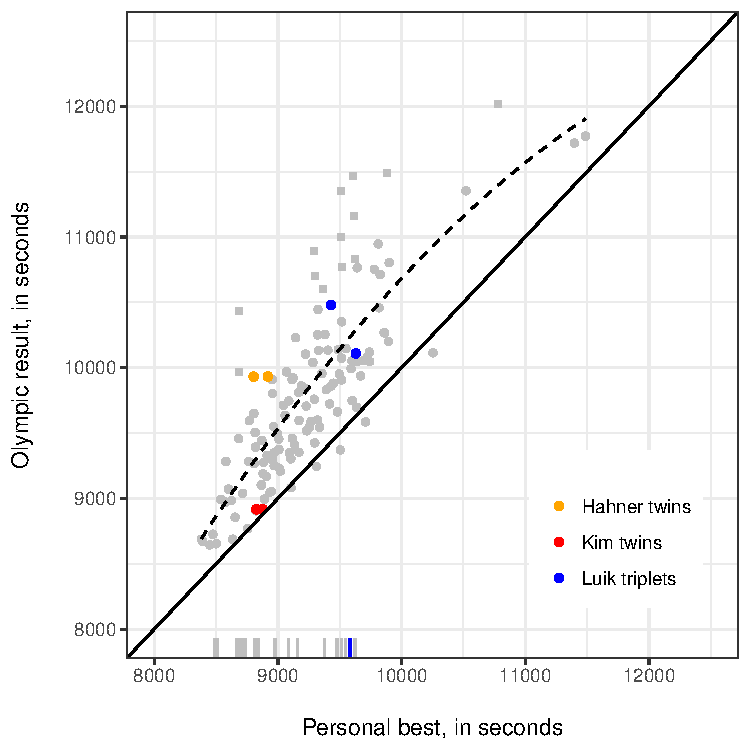
\includegraphics[width=\textwidth, keepaspectratio]{scatter_plot.pdf}
 \end{subfigure}
 \begin{subfigure}{.5\textwidth}
 %\label{fig:Studentized Residuals}
 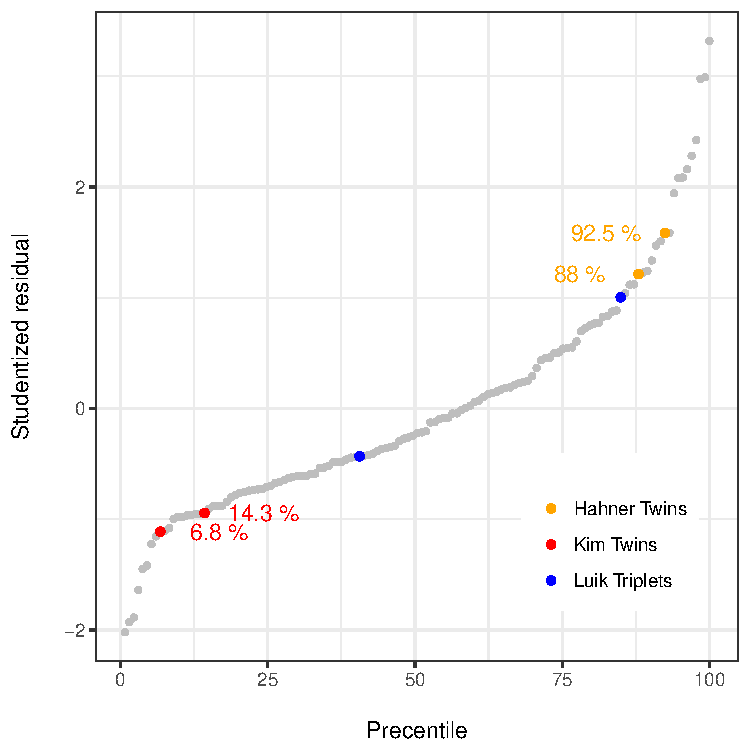
\includegraphics[width=.975\textwidth, keepaspectratio]{studentized_residuals.pdf}
 \end{subfigure}
\end{figure}

The scatter plot in Figure \ref{fig:scatter} displays the relationship between a runner's personal best and their final result.   Of the 156 runners that competed in the marathon event, 133 finished the race.  These individuals are plotted as grey points.  The 23 that did not finish are plotted below along the x-axis as grey tick-marks.   The dashed black line with grey confidence intervals represent OLS estimates of the linear relationship between the two variables.   The Hahner twins are marked by orange points. 

One can see that there is a clear linear relationship between a runner's performance in the olympics and her final result.  Moreover, there is a significant amount of noise in the relationship.  This suggests that despite one's innate abilities, luck plays a major role in olympic finishes.    Still, the twins' results are well above the fitted line, even accounting for typical error.  They are much slower than the underlying linear relationship suggests.  In fact, if we order each point by the size of the studentized residual (see the second plot), we can see that the Hahner twins are in the tail-end of the distribution.  Anna Hahner's residual deviation is greater than 91.7\% of the runners who completed the race while Lisa Hahner's deviation is greater than 86.5\%.  Hence, the twins appear to have finished at a much slower pace than expectation, which is what we might expect if they were coordinating their runs.\footnote{It is important to note that the North Korean twins finished much faster than expected.  XXXX explain PRK}   

\section*{Did Anna and Lisa intentionally finish together?}



\begin{figure}[!ht]
 \caption{Relationship between Difference in Personal Best and Difference in Result}
 \label{fig:diffdiff}
 \begin{subfigure}{.5\textwidth}
 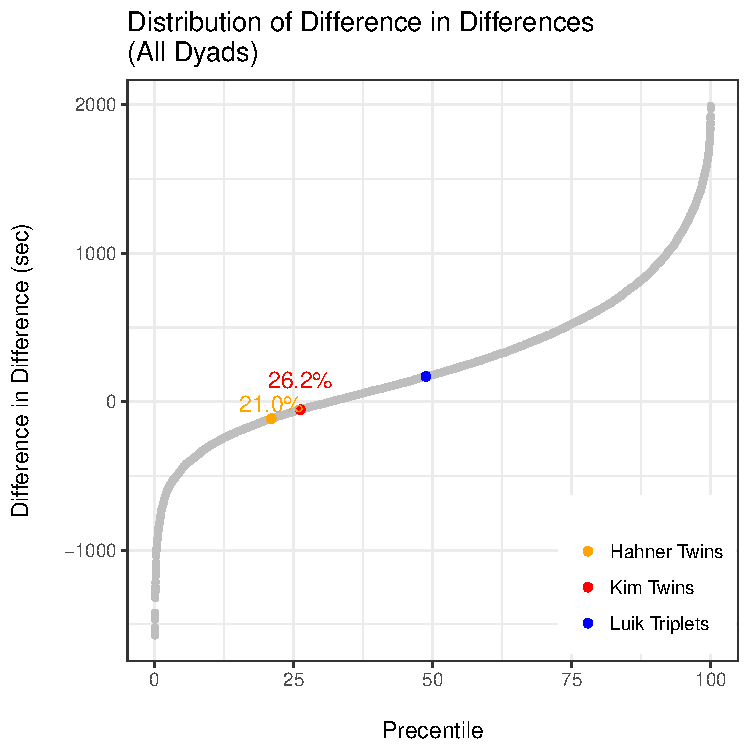
\includegraphics[width=\textwidth, keepaspectratio]{diff_in_diff_1.pdf}
 \end{subfigure}
 \begin{subfigure}{.5\textwidth}
 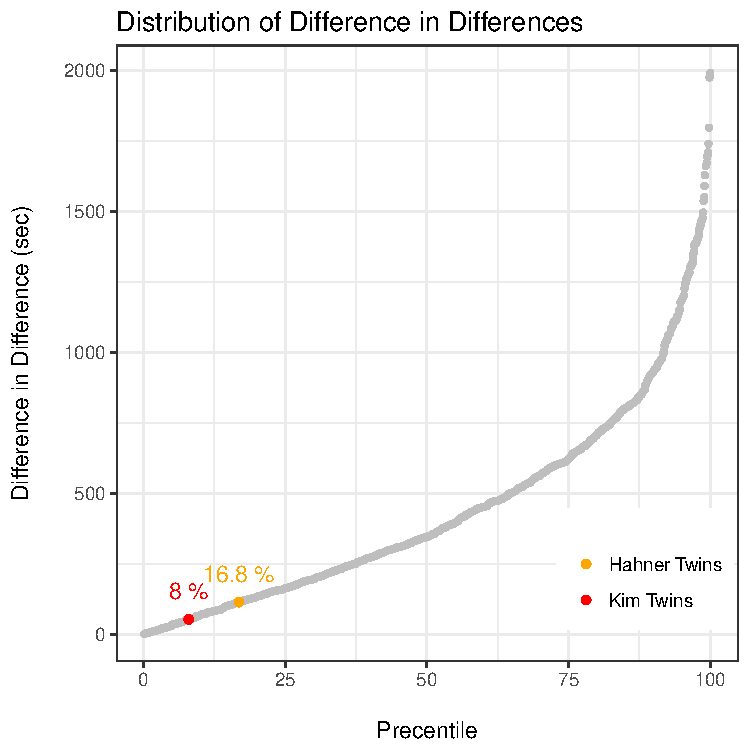
\includegraphics[width=\textwidth, keepaspectratio]{diff_in_diff_2.pdf}
 \end{subfigure}
\end{figure}

\newpage
\subsection*{Steps of the simulation}

\begin{enumerate}
\item Removing the twins from the sample, estimate a linear model that
predicts a runner?s final time ($Y_i$) based on her personal best time ($X_i$).
\item Extract the coefficients and the variance-covariance matrix from this
model.
\item For each runner, draw $\beta_0$ and $\beta_1$ from a multivariate normal
distribution with mean equal to the coefficients and variance equal to the
variance-covariance matrix.
\item For each runner, draw an error term ($e$) from a normal distribution with
mean equal to zero and a standard deviation equal to the standard
deviation of the model?s residuals ($\sigma$).
\item For each runner, predict the final result by combining the randomly
generated beta coefficients and error terms, $\hat{y} = \beta_0 + \beta_1 + e$.
\item Eliminate each runner from the race with a probability equal to the
percent of the total runners who did not finish in the actual race.  This
account for the likelihood of a DNF.
\item Calculate the difference in time between Anna Hahner and Lisa Hahner.
\item Calculate the difference in ranking between Anna Hahner and Lisa Hahner.
\item Repeat steps 3 through 8 ten thousand times.
\item Plot a histogram of the results in Figure \ref{fig:simdiff}
\end{enumerate}

\begin{figure}[!ht]
 \caption{The distribution of simulated results}
 \label{fig:simdiff}
 \begin{subfigure}{.5\textwidth}
 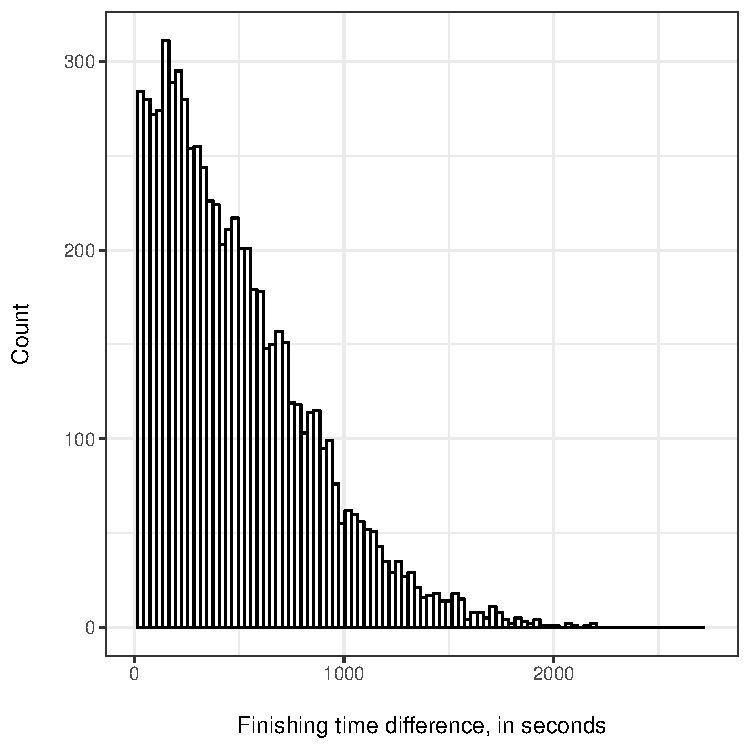
\includegraphics[width=\textwidth, keepaspectratio]{simulated_time.pdf}
 \end{subfigure}
 \begin{subfigure}{.5\textwidth}
 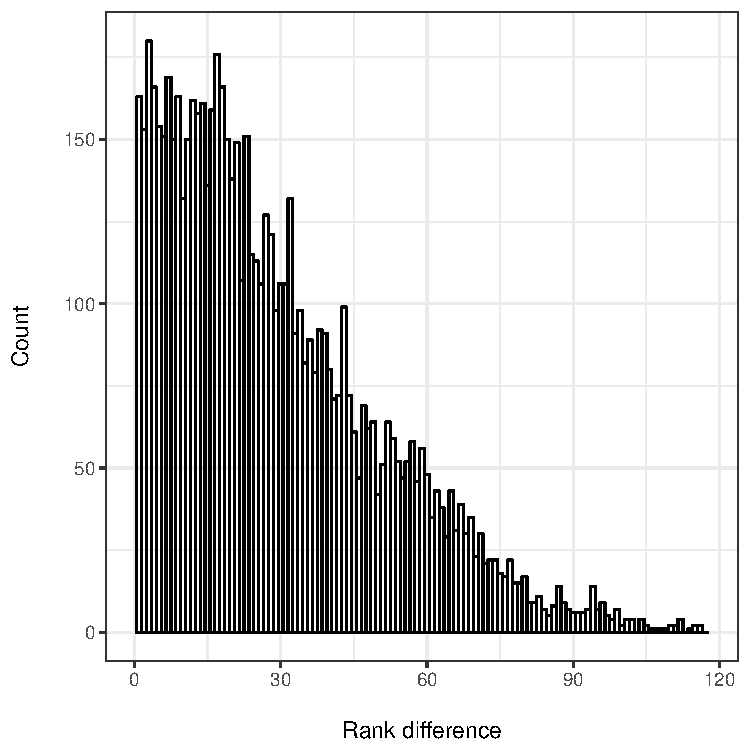
\includegraphics[width=\textwidth, keepaspectratio]{simulated_rank.pdf}
 \end{subfigure}
\end{figure}






   

\end{document}

